\section*{Model Overview}


In order to solve those problems, we will proceed as follows:

\begin{itemize}
    \begin{figure}[htbp]
        \centering
        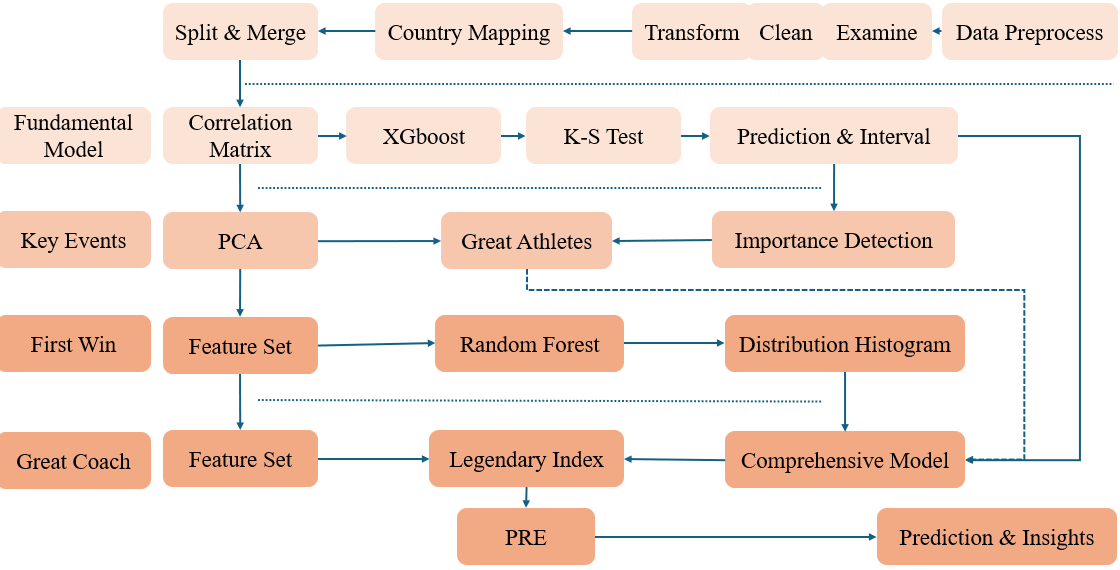
\includegraphics[width=1\textwidth]{./figures/figure1_work_flow.png}
        \caption{Flow chart}
        \label{fig:flow_chart}
    \end{figure}
    
\item {\bf Model Presentation}. We divide our task into four models: \textbf{Predicting the Medal of the 2028 LA Olympics}, \textbf{Key Events}, \textbf{Predicting First Medal Countries}, and \textbf{Great Coach Effect}.

\item {\bf Data Collection and Processing}. We gather relevant data, clean, and transform it. The data is then merged and analyzed using statistical methods to prepare it for machine learning.

\item {\bf Predictive Modeling}. We use various machine learning techniques, including \textbf{Random Forest} and \textbf{KS Test}, to build models that predict outcomes such as the first medal countries and key events.

\item {\bf Model Validation and Analysis}. We validate our models using statistical tests and analyze the performance of athletes and countries in specific sports/events. This includes forming the \textbf{Key Event Model} and the \textbf{Great Coach Model}.

\item {\bf Results and Discussion}. We present the results of our models, discuss their implications, and provide insights into the factors influencing the outcomes of the 2028 LA Olympics.
\end{itemize}
